\chapterimage{ampollxetas.png}
\chapter{Gestión Empresarial de seguridad de la información}
\begin{flushright}
    \textit{ }
\end{flushright}
%capítulo 4
%capítulo 11 12 13 14 15





%%%%%%%%%%%%%%%%%%%%%%%%%%%
%%%%%%%%%%%%%%%%%%%%%%%%%%%
%%%%%%%%%%%%%%%%%%%%%%%%%%%
\section{Seguridad Humana}
%%%%%%%%%%%%%%%%%%%%%%%%%%%
%%%%%%%%%%%%%%%%%%%%%%%%%%%
%%%%%%%%%%%%%%%%%%%%%%%%%%%
\color{blue}
\begin{itemize}
  \item Gestión de Identidad
  \item Ingeniería Social
  \item Cumplimiento Personal de las Reglas/Políticas/Normas Éticas de Ciberseguridad
  \item Conciencia y Comprensión
  \item Privacidad y Seguridad de Datos Personales
  \item Seguridad y Privacidad Utilizables
\end{itemize}
\color{black}

\subsection{Ética}
Proteger la sociedad, el bien común, la necesaria confianza y confianza pública y la infraestructura.
Actuar con honor, honestidad, justicia, responsabilidad y legalidad. =
Brindar un servicio diligente y competente a los directores.
Promover y proteger la profesión.
















%%%%%%%%%%%%%%%%%%%%%%%%
%%%%%%%%%%%%%%%%%%%%%%%%
%%%%%%%%%%%%%%%%%%%%%%%%
\section{Seguridad Organizacional}
%%%%%%%%%%%%%%%%%%%%%%%%
%%%%%%%%%%%%%%%%%%%%%%%%
%%%%%%%%%%%%%%%%%%%%%%%%
\color{blue}
\begin{itemize}
  \item Resultados de Aprendizaje de Seguridad Organizacional

  \item Gobierno y Políticas de Seguridad
  \item Herramientas Analíticas
  \item Administración de Sistemas
  \item Planificación de Ciberseguridad
   \item Gestión de Riesgos
   \item Continuidad del Negocio, Recuperación ante Desastres y Gestión de Incidentes
  \item Gestión de Programas de Seguridad
  \item Seguridad del Personal
\end{itemize}
\color{black}
En este capítulo nos centramos principalmente en la parte de disponibilidad de la tríada CIA y la importancia de mantener la disponibilidad para las operaciones comerciales. Esto es posible mediante la implementación de planes de Respuesta a incidentes, Continuidad comercial (BC) y/o Recuperación ante desastres (DR)

Primero, el plan de Respuesta a Incidentes responde a condiciones operativas anormales para mantener el negocio en funcionamiento. Los cuatro componentes principales de la Respuesta a Incidentes son: Preparación; Detección y Análisis; Contención, Erradicación y Recuperación; y Actividad Posterior al Incidente. Los equipos de respuesta a incidentes suelen ser un grupo multifuncional de personas que representan las áreas de responsabilidad administrativa, técnica y funcional más directamente afectadas por un incidente de seguridad. El equipo está capacitado en respuesta a incidentes y el plan de respuesta a incidentes de la organización. Cuando ocurre un incidente, el equipo es responsable de determinar la cantidad y el alcance del daño y si alguna información confidencial se vio comprometida, implementar procedimientos de recuperación para restaurar la seguridad y recuperarse del daño relacionado con el incidente, y supervisar la implementación de medidas futuras para mejorar la seguridad y prevenir reincidencia del incidente.

En segundo lugar, el plan de continuidad comercial está diseñado para mantener la organización en funcionamiento durante la crisis. Los componentes del plan de continuidad comercial incluyen detalles sobre cómo y cuándo implementar el plan y los sistemas de notificación y árboles de llamadas para alertar a los miembros del equipo y asociados de la organización que el plan ha sido implementado. Además, incluye números de contacto para comunicarse con socios externos críticos, proveedores de emergencia externos, vendedores y clientes. El plan proporciona al equipo procedimientos de respuesta inmediata y listas de verificación y orientación para la gestión.

Finalmente, cuando fallan los planes de Respuesta a Incidentes y Continuidad del Negocio (BC), se activa el plan de Recuperación ante Desastres (DR) para que las operaciones vuelvan a la normalidad lo más rápido posible. El plan de recuperación ante desastres (DR) puede incluir los siguientes componentes: resumen ejecutivo que proporciona una descripción general de alto nivel del plan, planes específicos de departamentos, guías técnicas para el personal de TI responsable de implementar y mantener sistemas críticos de respaldo, copias completas del plan para miembros críticos del equipo de recuperación ante desastres y listas de verificación para ciertas personas.
\subsection{Gestión de Riesgos}

 riesgo es una medida de la medida en que una entidad está amenazada por una circunstancia o evento potencial. A menudo se expresa como una combinación de:

los impactos adversos que surgirían si la circunstancia o evento ocurriera, y
la probabilidad de ocurrencia.

identificación de riesgos:

Identificar el riesgo para comunicarlo claramente.
Los empleados de todos los niveles de la organización son responsables de identificar los riesgos.
Identificar el riesgo para protegerse contra él


La probabilidad de ocurrencia es un factor ponderado basado en un análisis subjetivo de la probabilidad de que una determinada amenaza o conjunto de amenazas sea capaz de explotar una determinada vulnerabilidad o conjunto de vulnerabilidades.

 El impacto es la magnitud del daño que se puede esperar como resultado de las consecuencias de la divulgación no autorizada de información, la modificación no autorizada de información, la destrucción no autorizada de información o la pérdida de información o disponibilidad del sistema de información.





El riesgo de seguridad de la información refleja los impactos adversos potenciales que resultan de la posibilidad de acceso, uso, divulgación, interrupción, modificación o destrucción no autorizados de la información y/o los sistemas de información. Esta definición representa que el riesgo está asociado con amenazas, impacto y probabilidad, y también indica que el riesgo de TI es un subconjunto del riesgo empresaria

\begin{itemize}
    \item Un activo es algo que necesita protección.
    \item Una vulnerabilidad es una brecha o debilidad en esos esfuerzos de protección.
    \item Una amenaza es algo o alguien que tiene como objetivo explotar una vulnerabilidad para frustrar los esfuerzos de protección.

\end{itemize}

los actores de amenazas típicos    incluyen lo siguiente:

\begin{itemize}
    \item Insiders (ya sea deliberadamente, por simple error humano, o por incompetencia grave).
    \item Individuos externos o grupos informales (ya sea planificados u oportunistas, descubriendo la vulnerabilidad).
    \item Entidades formales que no son políticas (como competidores comerciales y ciberdelincuentes).
    \item Entidades formales que son políticas (como terroristas, estados-nación y hacktivistas).
    \item Recolectores de inteligencia o información (podría ser cualquiera de los anteriores).
    \item Tecnología (como bots de ejecución libre e inteligencia artificial, que podrían ser parte de cualquiera de los anteriores).

\end{itemize}
Vector de amenazas: Los medios por los cuales un actor de amenazas lleva a cabo sus objetivos.

Una vulnerabilidad es una debilidad o falla inherente en un sistema o componente que, si se desencadena o se actúa en consecuencia, podría causar que ocurra un evento de riesgo.

 La evaluación de riesgos se define como el proceso de identificar, estimar y priorizar los riesgos para las operaciones de una organización (incluida su misión, funciones, imagen y reputación), activos, personas, otras organizaciones e incluso la nación. La evaluación de riesgos debe resultar en alinear (o asociar) cada riesgo identificado que resulta de la operación de un sistema de información con las metas, objetivos, activos o procesos que utiliza la organización, lo que a su vez se alinea o respalda directamente el logro de las metas y objetivos de la organización.

 Un método eficaz para priorizar el riesgo es utilizar una matriz de riesgo, que ayuda a identificar la prioridad como la intersección de la probabilidad de ocurrencia y el impacto.

El tratamiento del riesgo se relaciona con la toma de decisiones sobre las mejores acciones a tomar con respecto al riesgo identificado y priorizado. Las decisiones que se toman dependen de la actitud de la gerencia hacia el riesgo y la disponibilidad, y el costo, de la mitigación del riesgo. Las opciones comúnmente utilizadas para responder al riesgo son:

\begin{itemize}
    \item Evitar el riesgo es la decisión de intentar eliminar el riesgo por completo. Esto podría incluir el cese de operaciones para algunas o todas las actividades de la organización que están expuestas a un riesgo particular. El liderazgo de la organización puede optar por evitar el riesgo cuando el impacto potencial de un riesgo dado es demasiado alto o si la probabilidad de que el riesgo se materialice es simplemente demasiado grande.
    \item La aceptación del riesgo es no tomar ninguna acción para reducir la probabilidad de que ocurra un riesgo. La gerencia puede optar por llevar a cabo la función comercial asociada con el riesgo sin ninguna otra acción por parte de la organización, ya sea porque el impacto o la probabilidad de ocurrencia es insignificante, o porque el beneficio es más que suficiente para compensar ese riesgo.
    \item La mitigación de riesgos es el tipo más común de gestión de riesgos e incluye la adopción de medidas para prevenir o reducir la posibilidad de un evento de riesgo o su impacto. La mitigación puede implicar medidas de remediación o controles, como controles de seguridad, establecimiento de políticas, procedimientos y estándares para minimizar el riesgo adverso. El riesgo no siempre se puede mitigar, pero siempre se deben implementar mitigaciones como las medidas de seguridad.
    \item La transferencia de riesgos es la práctica de pasar el riesgo a otra parte, quien aceptará el impacto financiero del daño resultante de la realización de un riesgo a cambio del pago. Por lo general, se trata de una póliza de seguro.
 \end{itemize}



\subsection{Continuidad del Negocio}


\begin{tcolorbox}[colback=gray!5!white,colframe=orange!60!gray,title=Caso]Imagine que el departamento de facturación de una empresa sufre una pérdida total en un incendio. El incendio ocurrió durante la noche, por lo que no había personal en el edificio en ese momento. Se realizó un Business Impact Analysis (BIA) hace cuatro meses e identificó las funciones del departamento de facturación como muy importantes para la empresa, pero que no afectan de inmediato a otras áreas de trabajo. Mediante un acuerdo previamente firmado, la empresa dispone de un área alternativa en la que puede trabajar el departamento de facturación, y que puede estar disponible en menos de una semana. Hasta que esa área pueda estar completamente lista, las consultas de facturación de los clientes serán respondidas por el personal de servicio al cliente. El personal del departamento de facturación permanecerá en el área alterna de trabajo hasta que se disponga de una nueva área permanente.
\end{tcolorbox}


Componentes comunes de un plan integral de continuidad del negocio:
\begin{itemize}
    \item Lista de los miembros del equipo BCP, incluidos múltiples métodos de contacto y miembros de respaldo
    \item Procedimientos de respuesta inmediata y listas de verificación (procedimientos de seguridad y protección, procedimientos de supresión de incendios, notificación de las agencias de respuesta de emergencia apropiadas, etc.)
    \item Sistemas de notificación y árboles de llamadas para alertar al personal de que se está promulgando el BCP
    \item Orientación para la gestión, incluida la designación de autoridad para gerentes específicos
    \item Cómo/cuándo promulgar el plan
    \item Números de contacto de miembros críticos de la cadena de suministro (proveedores, clientes, posibles proveedores externos de emergencia, socios externos)


\end{itemize}

\subsection{Recuperación ante Desastres y Gestión de Incidentes}


\begin{tcolorbox}[colback=gray!5!white,colframe=orange!60!gray,title=Caso]En un hospital de Los Ángeles, tomó 260 días (alrededor de 8 meses y medio) para descubrir que había un compromiso. En este caso, el hospital no pudo volver a hacer negocios utilizando la última copia de seguridad porque estaba plagado de un malware basado en el tiempo que corrompería todos los datos en el sistema tan pronto como se restaurara. El hospital necesitaba retroceder casi un año antes de descubrir el incidente para restaurar todo el sistema y luego restaurar los datos restantes pieza por pieza para evitar la reinfección. Este escenario destaca la necesidad de varios niveles de respaldo y períodos de retención para abordar las necesidades de la organización.
\end{tcolorbox}
\begin{figure}[H]
    \centering
    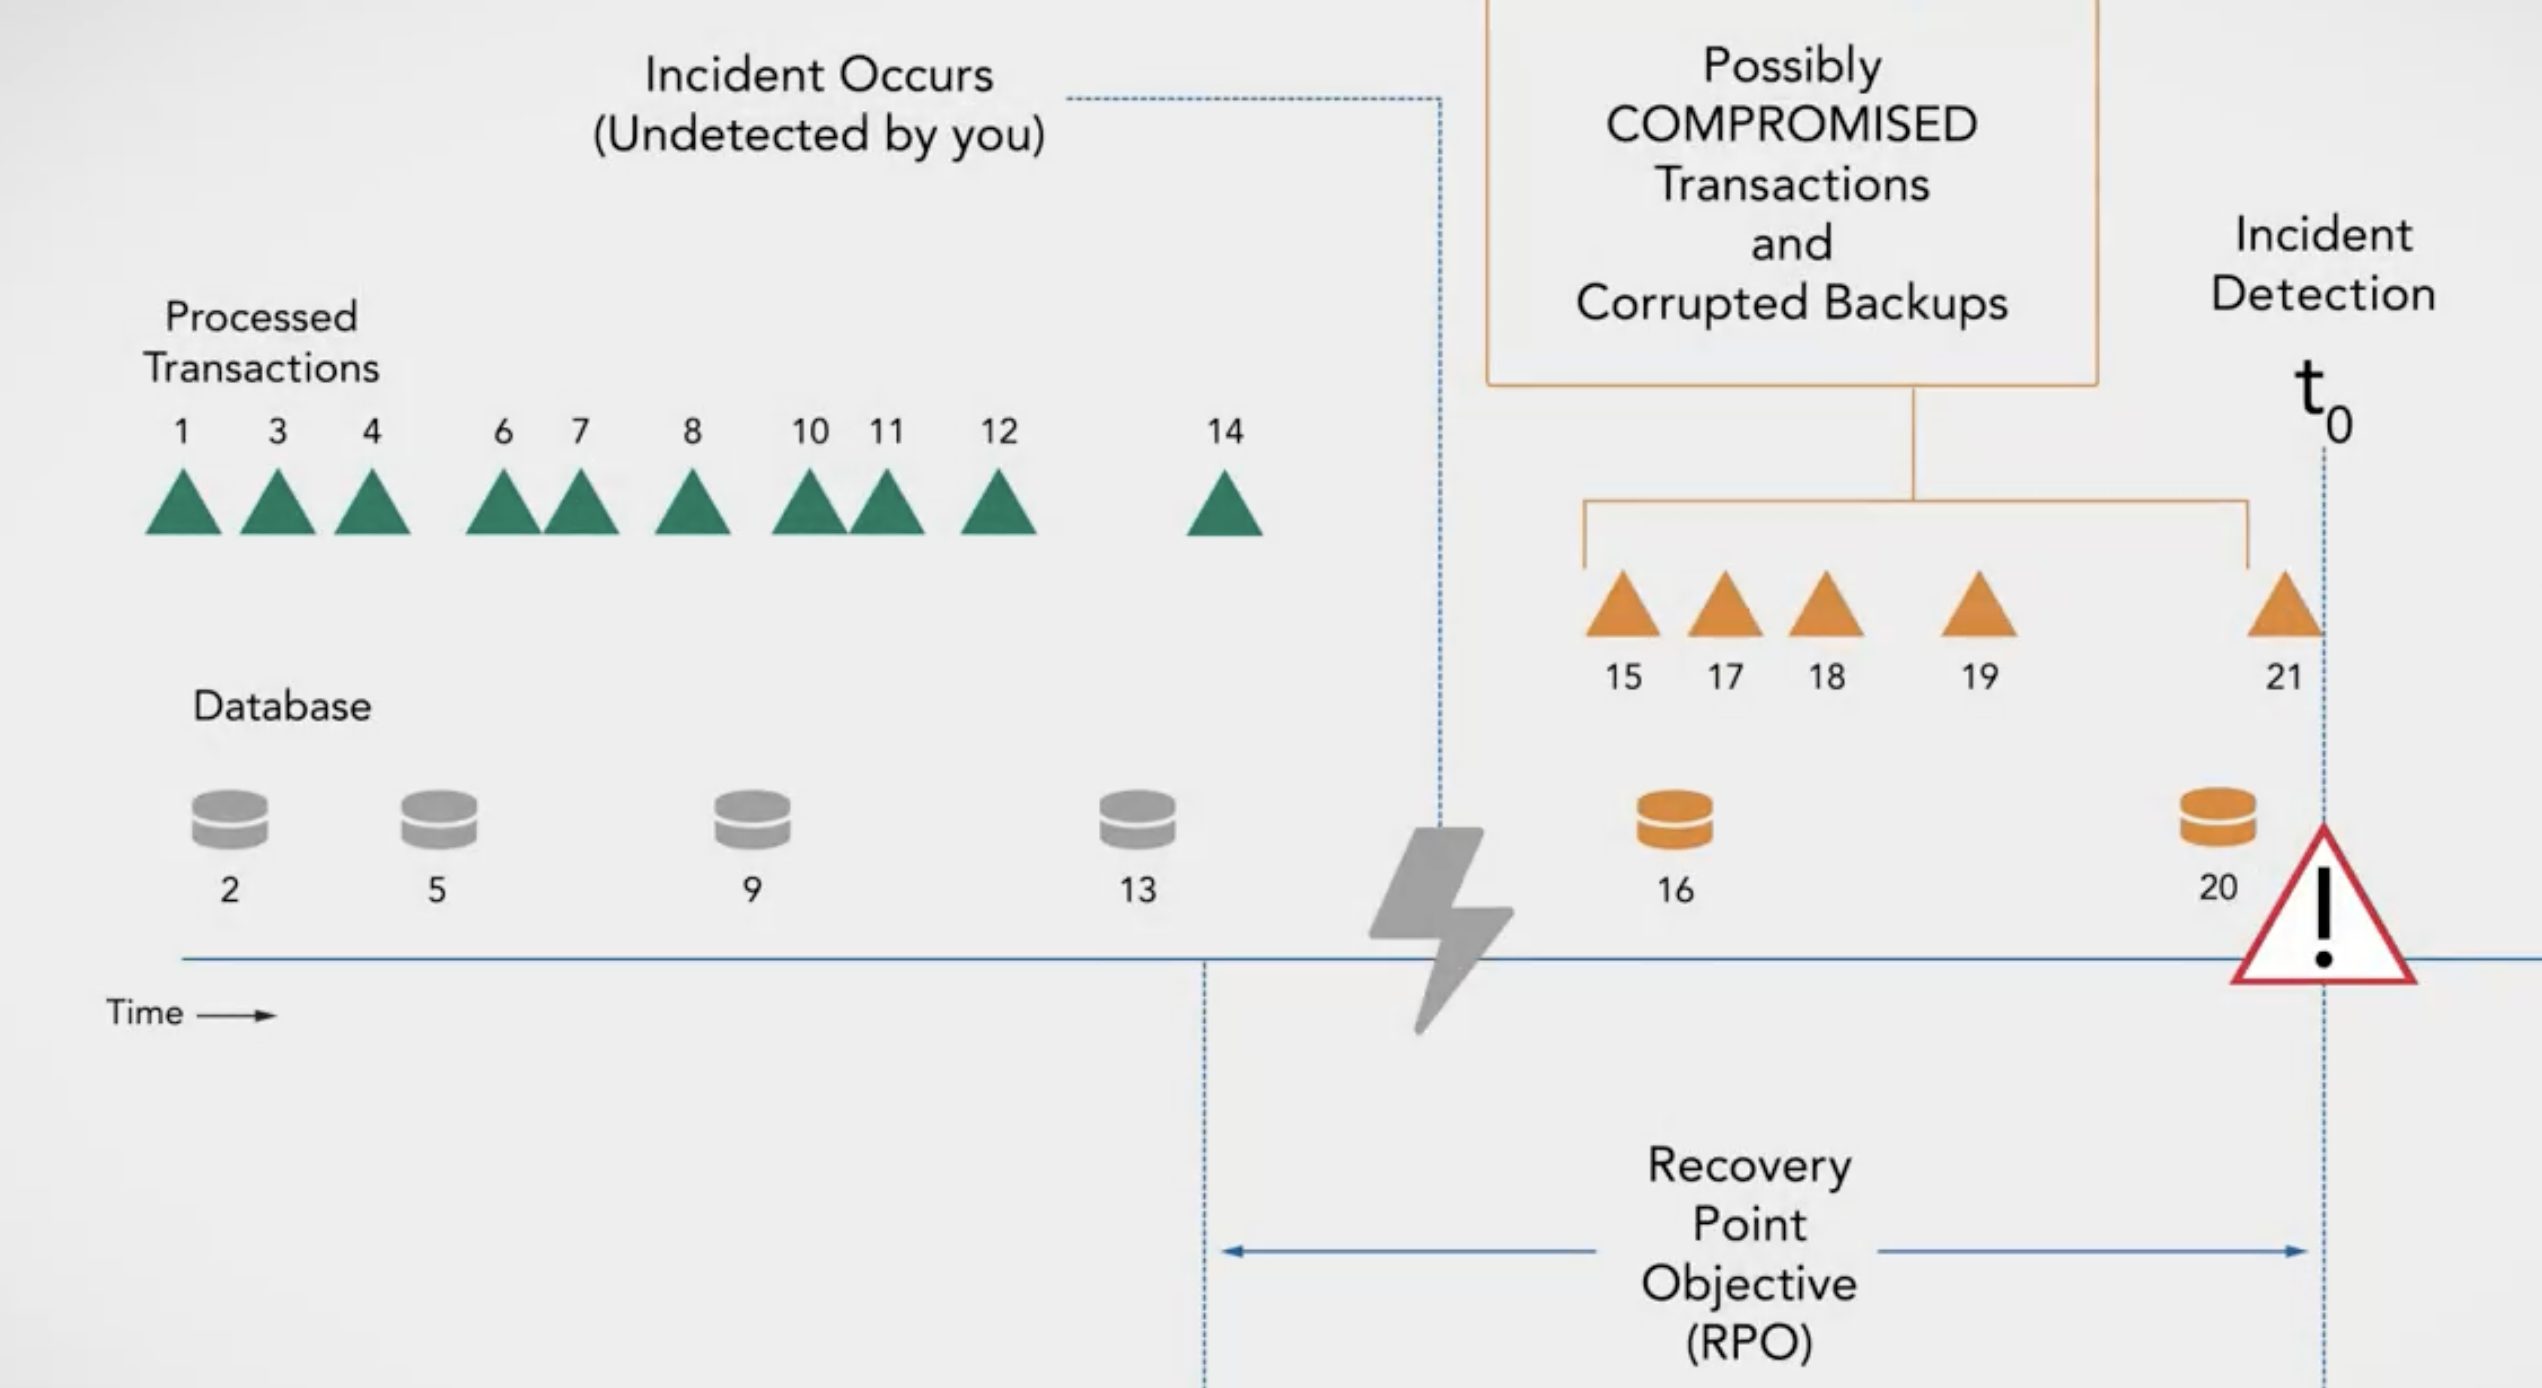
\includegraphics[scale=0.3]{imgs/ataquepuntorecuperacion.png}
    \caption{Descubriendo hasta cuando debemos devolvernos. Fuente externa}
    \label{fig:enter-label}
\end{figure}
\begin{comment}
    Un ejemplo de recuperación ante desastres en acción es el uso de copias de seguridad del sistema. La línea de tiempo de esta imagen mira hacia atrás en el tiempo desde el momento de la detección del incidente (a la derecha) como una forma de identificar la cantidad de trabajo que se perderá al recargar desde una copia de seguridad. Los eventos de procesamiento de transacciones (los triángulos) y algunos eventos de copia de seguridad (que se muestran como símbolos de la base de datos) se han numerado como eventos del 1 al 21 de izquierda a derecha a lo largo de la línea de tiempo. Las transacciones verdes (eventos 1 a 14) son las que se procesaron por completo antes de la intrusión o el inicio del incidente. Presumiblemente, y si el antivirus y otros sistemas funcionan correctamente, esta puede ser una suposición segura. Estas transacciones no estuvieron expuestas a una posible pérdida de integridad, autenticidad, privacidad o cualquier otro atributo de seguridad requerido.

Los símbolos de la base de datos que se muestran en gris (eventos 2, 5, 9 y 13, todos anteriores al evento) representan alguna forma de sistema y respaldo de datos que pueden haber capturado los cambios en el sistema como resultado de completar correctamente las transacciones verdes.

Sin embargo, son los eventos 15 a 21 los que están en duda. Pueden estar bien o pueden representar una falta de integridad si los datos se vieron comprometidos. Los símbolos de copia de seguridad de la base de datos en color naranja, entre el momento de la ocurrencia de la incidencia y su detección, están claramente en duda en cuanto a su integridad o seguridad. Pueden contener datos falsos, corruptos o incluso pueden contener malware en una variedad de formas. Retrocediendo en el tiempo desde la detección del incidente, no es hasta que llegamos al símbolo gris de la base de datos más a la derecha (evento 13, la copia de seguridad justo antes de que ocurra el incidente) que tenemos nuestra última copia de seguridad limpia y confiable.

Se pueden identificar tres conjuntos de trabajo que se perdieron desde que comenzó a ocurrir el incidente: todas las transacciones o cambios anteriores a la última copia de seguridad correcta que no formaban parte de esa copia de seguridad, si era una copia de seguridad incremental o parcial y no una copia de seguridad completa, eventos 15, 17 a 19 y 21; todas las transacciones y otros cambios procesados o intentados desde esa copia de seguridad en el tiempo hasta después de que se detectó el incidente, no comenzaron a ocurrir; y todos los cambios de transacciones, etc. que normalmente se habrían procesado desde el momento en que se detectó el incidente hasta que el sistema volvió a estar completamente operativo, pero que no pudieron procesarse en absoluto debido a la interrupción.
\end{comment}

El plan de recuperación ante desastres (DRP) guía las acciones del personal de respuesta a emergencias hasta que se alcance el objetivo final, que es ver que el negocio se restablezca a las últimas operaciones confiables conocidas. Se refiere a la \textbf{restauración de los servicios y sistemas de tecnología de la información y comunicaciones que necesita una organización, tanto durante el período de interrupción causado por cualquier evento como durante la restauración de los servicios normales.} La recuperación de TI suele ser crucial para la recuperación y el sostenimiento de las operaciones comerciales. 














\section{Seguridad Defensiva}
\color{blue}
Tareas principales:
\begin{itemize}
\item Evitar que se produzcan intrusiones
\item Detectar intrusiones cuando ocurren y responder adecuadamente
\end{itemize}

subtareas:

\begin{itemize}
\item \textbf{Conciencia de seguridad cibernética del usuario}: capacitar a los usuarios sobre seguridad cibernética ayuda a proteger contra varios ataques que tienen como objetivo sus sistemas.
\item \textbf{Documentación y gestión de activos}: Necesitamos conocer los tipos de sistemas y dispositivos que tenemos que gestionar y proteger adecuadamente.
\item \textbf{Actualización y parcheo de sistemas}: Asegurar que las computadoras, servidores y dispositivos de red estén correctamente actualizados y parcheados contra cualquier vulnerabilidad conocida (debilidad).
\item  \textbf{Configuración de dispositivos de seguridad preventiva}: el \textbf{firewall} y los \textbf{sistemas de prevención de intrusos} ( IPS ) son componentes críticos de la seguridad preventiva. \textit{Los cortafuegos controlan qué tráfico de red puede entrar y qué puede salir del sistema o la red}. \textit{IPS bloquea cualquier tráfico de red que coincida con las reglas actuales y las \textbf{firmas de ataque}.}
\item  \textbf{Configuración de dispositivos de registro y monitoreo}: sin un registro y monitoreo adecuados de la red, no será posible detectar actividades maliciosas e intrusiones. Si aparece un nuevo dispositivo no autorizado en nuestra red, deberíamos poder saberlo.
\end{itemize}
\color{black}




\subsection{Centro de Operaciones de Seguridad ( SOC )}
Un Centro de Operaciones de Seguridad ( SOC ) es un equipo de profesionales de seguridad cibernética que \textbf{monitorea la red y sus sistemas para detectar eventos maliciosos de seguridad cibernética}. Algunas de las principales áreas de interés para un SOC son:
\begin{itemize}
\item \textbf{Vulnerabilidades}: cada vez que se descubre una vulnerabilidad del sistema (debilidad), es esencial repararla instalando una actualización o parche adecuado. \textbf{Cuando una solución no está disponible, se deben tomar las medidas necesarias para evitar que un atacante la explote}. Aunque la reparación de vulnerabilidades es de vital interés para un SOC , no necesariamente se les asigna.
\item \textbf{Violaciones de políticas}: podemos pensar en una \textbf{política de seguridad como un conjunto de reglas necesarias para la protección de la red y los sistemas}. Por ejemplo, podría ser una violación de la política si los usuarios comienzan a cargar datos confidenciales de la empresa en un servicio de almacenamiento en línea.
\item \textbf{Actividad no autorizada}: considere el caso en el que se roban el nombre de inicio de sesión y la contraseña de un usuario, y el atacante los usa para iniciar sesión en la red. Un SOC necesita detectar tal evento y bloquearlo lo antes posible antes de que se produzcan más daños.

\item \textbf{Intrusiones en la red}: Una intrusión puede ocurrir cuando un usuario hace clic en un enlace malicioso o cuando un atacante explota un servidor público. De cualquier manera, cuando se produce una intrusión, debemos detectarla lo antes posible para evitar daños mayores.
\end{itemize}

La Inteligencia de amenazas es otra tarea del SOC y hace referencia  a la información que recopila sobre enemigos reales y potenciales. \textbf{Una amenaza es cualquier acción que puede interrumpir o afectar negativamente a un sistema}. La inteligencia de amenazas tiene como objetivo recopilar información para ayudar a la empresa a prepararse mejor contra posibles adversarios. El propósito sería lograr una defensa informada por la amenaza . Diferentes empresas tienen diferentes adversarios. Algunos adversarios podrían intentar robar datos de clientes de un operador móvil; sin embargo, otros adversarios están interesados en detener la producción en una refinería de petróleo. Los adversarios de ejemplo incluyen un ejército cibernético de un estado-nación que trabaja por razones políticas y un grupo de ransomware que actúa con fines financieros. 

La inteligencia necesita datos. Los datos tienen que ser recopilados, procesados y analizados. La recopilación de datos se realiza a partir de fuentes locales, como registros de red, y fuentes públicas, como foros. El procesamiento de datos tiene como objetivo organizarlos en un formato adecuado para el análisis. La fase de análisis busca encontrar \textbf{más información sobre los atacantes y sus motivos}; conocer sus \textbf{tácticas, técnicas y procedimientos} para 1) identificar  al actor de amenazas (adversario), 2) predecir su actividad y, 3) en consecuencia, podremos mitigar sus ataques y 4) preparar una estrategia de respuesta.

La ciencia Forense digital es la aplicación de la ciencia para investigar delitos y establecer hechos. Con el uso y la difusión de los sistemas digitales, como computadoras y teléfonos inteligentes, nació una nueva rama de la ciencia forense para investigar delitos relacionados: la ciencia forense informática, que más tarde se convirtió en ciencia forense digital .

En la seguridad defensiva, el enfoque del análisis forense digital cambia al análisis de la evidencia de un ataque y sus perpetradores y otras áreas como el robo de propiedad intelectual, el espionaje cibernético y la posesión de contenido no autorizado. En consecuencia, el análisis forense digital se centrará en diferentes áreas, tales como:
\begin{itemize}
\item \textbf{Sistema de archivos}: el análisis de una imagen forense digital (copia de bajo nivel) del almacenamiento de un sistema revela mucha información, como programas instalados, archivos creados, archivos sobrescritos parcialmente y archivos eliminados.
\item \textbf{Memoria del sistema}: si el atacante está ejecutando su programa malicioso en la memoria sin guardarlo en el disco, tomar una imagen forense (copia de bajo nivel) de la memoria del sistema es la mejor manera de analizar su contenido y aprender sobre el ataque.
\item \textbf{Registros del sistema}: cada computadora cliente y servidor mantiene diferentes archivos de registro sobre lo que está sucediendo. Los archivos de registro proporcionan mucha información sobre lo que sucedió en un sistema. Se dejarán algunos rastros incluso si el atacante intenta borrar sus rastros.
\item \textbf{Registros de red}: los registros de los paquetes de red que han atravesado una red ayudarían a responder más preguntas sobre si se está produciendo un ataque y qué implica.
\end{itemize}


Un incidente generalmente se refiere a una violación de datos o un ataque cibernético; sin embargo, en algunos casos, puede ser algo menos crítico, como una mala configuración, un intento de intrusión o una violación de la política. Los ejemplos de un ataque cibernético incluyen un atacante que hace que nuestra red o sistemas sean inaccesibles, desfigurar (cambiar) el sitio web público y la violación de datos (robar datos de la empresa). ¿ Cómo responderías a un ciberataque? La respuesta a incidentes especifica la metodología que debe seguirse para manejar tal caso. El objetivo es \textbf{reducir los daños y recuperarse en el menor tiempo posible}. Idealmente, desarrollaría un plan listo para la respuesta a incidentes.

Las cuatro fases principales del proceso de respuesta a incidentes son:

\begin{itemize}
\item \textbf{Preparación}: Esto requiere un equipo capacitado y listo para manejar incidentes. Idealmente, se implementan varias medidas para evitar que ocurran incidentes en primer lugar.
\item \textbf{Detección y Análisis}: El equipo cuenta con los recursos necesarios para detectar cualquier incidencia; además, es fundamental profundizar en el análisis de cualquier incidente detectado para conocer su gravedad.
\item \textbf{Contención, erradicación y recuperación}: una vez que se detecta un incidente, es crucial evitar que afecte a otros sistemas, eliminarlo y recuperar los sistemas afectados. Por ejemplo, cuando notamos que un sistema está infectado con un virus informático, nos gustaría evitar (contener) que el virus se propague a otros sistemas, limpiar (erradicar) el virus y garantizar una recuperación adecuada del sistema.
\item \textbf{Actividad posterior al incidente}: después de una recuperación exitosa, se genera un informe y se comparte la lección aprendida para evitar incidentes similares en el futuro.
\end{itemize}

\subsection{Inteligencia de Amenazas}

En este contexto, la inteligencia se refiere a la información que recopilas sobre enemigos reales y potenciales. \textbf{Una amenaza es cualquier acción que puede interrumpir o afectar negativamente a un sistema}. La inteligencia de amenazas tiene como objetivo recopilar información para ayudar a la empresa a prepararse mejor contra posibles adversarios. El propósito sería lograr una defensa informada por la amenaza . Diferentes empresas tienen diferentes adversarios. Algunos adversarios podrían intentar robar datos de clientes de un operador móvil; sin embargo, otros adversarios están interesados en detener la producción en una refinería de petróleo. Los adversarios de ejemplo incluyen un ejército cibernético de un estado-nación que trabaja por razones políticas y un grupo de ransomware que actúa con fines financieros. Según la empresa (objetivo), podemos esperar adversarios.

La inteligencia necesita datos. Los datos tienen que ser recopilados, procesados y analizados. La recopilación de datos se realiza a partir de fuentes locales, como registros de red, y fuentes públicas, como foros. El \textbf{procesamiento de datos } tiene como objetivo organizarlos en un formato adecuado para el análisis. La fase de \textbf{análisis} busca encontrar más información sobre los atacantes y sus motivos; además, tiene como objetivo crear una lista de recomendaciones y pasos prácticos.

Aprender sobre tus adversarios te permite conocer sus \textbf{tácticas, técnicas y procedimientos}. Como resultado de la inteligencia de amenazas, identificamos al actor de amenazas (adversario), predecimos su actividad y, en consecuencia, podremos mitigar sus ataques y preparar una estrategia de respuesta.


\subsection{Controles de seguridad}
Los controles de seguridad pertenecen a los mecanismos físicos, técnicos y administrativos que actúan como salvaguardas o contramedidas prescritas para un sistema de información para proteger la confidencialidad, integridad y disponibilidad del sistema y su información. La implementación de controles debería reducir el riesgo.

Los controles físicos abordan las necesidades de seguridad basadas en procesos utilizando dispositivos de hardware físico, como lectores de tarjetas, características arquitectónicas de edificios e instalaciones y acciones de seguridad específicas que deben tomar las personas. Por lo general, brindan formas de controlar, dirigir o prevenir el movimiento de personas y equipos en una ubicación física específica, como una oficina, una fábrica u otra instalación. Los controles físicos también brindan protección y control sobre la entrada al terreno que rodea los edificios, estacionamientos u otras áreas que están bajo el control de la organización. En la mayoría de las situaciones, los controles físicos están respaldados por controles técnicos como un medio para incorporarlos a un sistema de seguridad general.

Los controles técnicos (también llamados controles lógicos) son controles de seguridad que los sistemas informáticos y las redes implementan directamente. Estos controles pueden brindar protección automatizada contra el acceso no autorizado o el uso indebido, facilitar la detección de violaciones de seguridad y respaldar los requisitos de seguridad para aplicaciones y datos. Los controles técnicos pueden ser ajustes de configuración o parámetros almacenados como datos, administrados a través de una interfaz gráfica de usuario (GUI) de software, o pueden ser ajustes de hardware realizados con interruptores, puentes u otros medios. Sin embargo, la implementación de controles técnicos siempre requiere importantes consideraciones operativas y debe ser coherente con la gestión de la seguridad dentro de la organización

Los controles administrativos (también conocidos como controles gerenciales) son directivas, lineamientos o avisos dirigidos a las personas dentro de la organización. Proporcionan marcos, restricciones y estándares para el comportamiento humano, y deben cubrir todo el alcance de las actividades de la organización y sus interacciones con partes externas y partes interesadas.




%%%%%%%%%%%%%%%%%%%%%%%%%%%%%
%%%%%%%%%%%%%%%%%%%%%%%%%%%%%
%%%%%%%%%%%%%%%%%%%%%%%%%%%%%
\subsection{Respuesta al incidente}
%%%%%%%%%%%%%%%%%%%%%%%%
%%%%%%%%%%%%%%%%%%%%%%%%
%%%%%%%%%%%%%%%%%%%%%%%%
Un incidente generalmente se refiere a una violación de datos o un ataque cibernético; sin embargo, en algunos casos, puede ser algo menos crítico, como una mala configuración, un intento de intrusión o una violación de la política. Los ejemplos de un ataque cibernético incluyen un atacante que hace que nuestra red o sistemas sean inaccesibles, desfigurar (cambiar) el sitio web público y la violación de datos (robar datos de la empresa). 


El objetivo principal de la gestión de incidentes es estar preparado. La preparación requiere tener una política y un plan de respuesta que guíe a la organización a través de la crisis. Cada organización debe tener un plan de respuesta a incidentes que ayudará a preservar la viabilidad y supervivencia del negocio.

Las cuatro fases principales del \textbf{proceso de respuesta a incidentes} el cual tiene por objetivo reducir el impacto de un incidente para que la organización pueda reanudar las operaciones interrumpidas lo antes posible, son:
\begin{itemize}
    \item \textbf{Preparación}: Esto requiere un equipo capacitado y listo para manejar incidentes. Idealmente, se implementan varias medidas para evitar que ocurran incidentes en primer lugar.
    \begin{itemize}
        \item Desarrollar una política aprobada por la gerencia.
        \item Identifique datos y sistemas críticos, puntos únicos de falla.
        \item Capacitar al personal en la respuesta a incidentes.
        \item Implementar un equipo de respuesta a incidentes. 
        \item Practique la identificación de incidentes. (Primera respuesta)
        \item Identificar roles y responsabilidades.
        \item Planificar la coordinación de la comunicación entre las partes interesadas.
        \item Considere la posibilidad de que un método principal de comunicación no esté disponible.
    \end{itemize}
\item \textbf{Detección y Análisis}: El equipo cuenta con los recursos necesarios para detectar cualquier incidencia; además, es fundamental profundizar en el análisis de cualquier incidente detectado para conocer su gravedad.
    \begin{itemize}
        \item Supervise todos los posibles vectores de ataque.
        \item Analice incidentes utilizando datos conocidos e inteligencia de amenazas.
        \item Priorizar la respuesta a incidentes.
        \item Estandarizar la documentación de incidentes.
    \end{itemize}
\textbf{Contención, erradicación y recuperación}: una vez que se detecta un incidente, es crucial evitar que afecte a otros sistemas, eliminarlo y recuperar los sistemas afectados. Por ejemplo, cuando notamos que un sistema está infectado con un virus informático, nos gustaría evitar (contener) que el virus se propague a otros sistemas, limpiar (erradicar) el virus y garantizar una recuperación adecuada del sistema.
\begin{itemize}
    \item Reunir evidencias.
    \item Elija una estrategia de contención adecuada.
    \item Identificar al atacante.
    \item Aislar el ataque.
\end{itemize}
\textbf{Actividad posterior al incidente}: después de una recuperación exitosa, se genera un informe y se comparte la lección aprendida para evitar incidentes similares en el futuro.
\begin{itemize}
    \item Identificar la evidencia que puede ser necesario conservar.
\item Documentar las lecciones aprendidas.
\end{itemize}
\end{itemize}

Un equipo típico de respuesta a incidentes es un grupo interdisciplinario de personas que representan las áreas de responsabilidad gerencial, técnica y funcional más directamente afectadas por un incidente de seguridad. Los miembros potenciales del equipo incluyen lo siguiente:

\begin{itemize}
    \item Representante(s) de la alta gerencia
    \item Profesionales de la seguridad de la información
    \item Representantes legales
    \item Representantes de asuntos públicos/comunicaciones
Representantes de ingeniería (sistema y red)

\end{itemize}







\section{Análisis de malware}
Malware significa software malicioso. El software se refiere a programas, documentos y archivos que puede guardar en un disco o enviar a través de la red. El malware incluye muchos tipos, como:
\begin{itemize}
Un \textbf{virus} es una pieza de código (parte de un programa) que se adjunta a un programa. Está diseñado para propagarse de una computadora a otra; además, funciona modificando, sobrescribiendo y eliminando archivos una vez que infecta una computadora. El resultado varía desde que la computadora se vuelve lenta hasta inutilizable.
\item \textbf{Trojan Horse} es un programa que muestra una función deseable pero oculta una función maliciosa debajo. Por ejemplo, una víctima puede descargar un reproductor de video de un sitio web dudoso que le da al atacante un control total sobre su sistema.
\item El \textbf{ransomware} es un programa malicioso que cifra los archivos del usuario. El cifrado hace que los archivos sean ilegibles sin conocer la contraseña de cifrado. El atacante ofrece al usuario la contraseña de cifrado si el usuario está dispuesto a pagar un "rescate".
\end{itemize}

El análisis de malware tiene como objetivo aprender acerca de dichos programas maliciosos utilizando varios medios:
\begin{itemize}
\item El \textbf{análisis estático} funciona al inspeccionar el programa malicioso sin ejecutarlo. Por lo general, esto requiere un conocimiento sólido del lenguaje ensamblador (conjunto de instrucciones del procesador, es decir, las instrucciones fundamentales de la computadora).
\item El \textbf{análisis dinámico} funciona ejecutando el malware en un entorno controlado y monitoreando sus actividades. Le permite observar cómo se comporta el malware cuando se ejecuta.\end{itemize}



\subsection{Forense digital}
La ciencia forense es la aplicación de la ciencia para investigar delitos y establecer hechos. Con el uso y la difusión de los sistemas digitales, como computadoras y teléfonos inteligentes, nació una nueva rama de la ciencia forense para investigar delitos relacionados: la \textbf{ciencia forense informática}, que más tarde se convirtió en \textbf{ciencia forense digital}.

En la seguridad defensiva, el enfoque del análisis forense digital cambia al análisis de la evidencia de un ataque y sus perpetradores y otras áreas como el robo de propiedad intelectual, el espionaje cibernético y la posesión de contenido no autorizado. En consecuencia, el análisis forense digital se centrará en diferentes áreas, tales como:
\begin{itemize}
    \item  Sistema de archivos: el análisis de una imagen forense digital (copia de bajo nivel) del almacenamiento de un sistema revela mucha información, como programas instalados, archivos creados, archivos sobrescritos parcialmente y archivos eliminados.
\item Memoria del sistema: si el atacante está ejecutando su programa malicioso en la memoria sin guardarlo en el disco, tomar una imagen forense (copia de bajo nivel) de la memoria del sistema es la mejor manera de analizar su contenido y aprender sobre el ataque.
\item Registros del sistema: cada computadora cliente y servidor mantiene diferentes archivos de registro sobre lo que está sucediendo. Los archivos de registro proporcionan mucha información sobre lo que sucedió en un sistema. Se dejarán algunos rastros incluso si el atacante intenta borrar sus rastros.
\item Registros de red: los registros de los paquetes de red que han atravesado una red ayudarían a responder más preguntas sobre si se está produciendo un ataque y qué implica.

\end{itemize}




%%%%%%%%%%%%%%%%%%%%%%%%%%%%%%%%%
%%%%%%%%%%%%%%%%%%%%%%%%%%%%%%%%%
%%%%%%%%%%%%%%%%%%%%%%%%%%%%%%%%%
\section{Seguridad Societal}
%%%%%%%%%%%%%%%%%%%%%%%%
%%%%%%%%%%%%%%%%%%%%%%%%
%%%%%%%%%%%%%%%%%%%%%%%%
\color{blue}
\begin{itemize}
  \item Resultados de Aprendizaje de Seguridad Societal
  \item Ciberdelincuencia
  \item Legislación en Ciberseguridad
  \item Ética en Ciberseguridad
  \item Políticas de Ciberseguridad
  \item Privacidad
\end{itemize}
\color{black}
\subsection{Gobernanza}
Los procedimientos son los pasos detallados para completar una tarea que respaldan las políticas departamentales u organizacionales.
Las políticas son implementadas por el gobierno de la organización, como la dirección ejecutiva, para brindar orientación en todas las actividades para garantizar que la organización cumpla con los estándares y regulaciones de la industria.
Los equipos de gobierno a menudo utilizan los estándares para proporcionar un marco para introducir políticas y procedimientos en apoyo de las regulaciones.
Las regulaciones se emiten comúnmente en forma de leyes, generalmente del gobierno (que no debe confundirse con la gobernanza) y generalmente conllevan sanciones financieras por incumplimiento

Reglamentos y Leyes

Los gobiernos pueden imponer regulaciones y multas y sanciones asociadas a nivel nacional, regional o local.


La Ley de Portabilidad y Responsabilidad de Seguros Médicos (HIPAA) de 1996 es un ejemplo de una ley que rige el uso de la información médica protegida (PHI) en los Estados Unidos. La violación de la regla HIPAA conlleva la posibilidad de multas y/o encarcelamiento tanto para individuos como para empresas.

El Reglamento General de Protección de Datos (RGPD) fue promulgado por la Unión Europea (UE) para controlar el uso de la Información de Identificación Personal (PII) de sus ciudadanos y los de la UE. Incluye disposiciones que aplican sanciones económicas a las empresas que manejan datos de ciudadanos de la UE y residentes en la UE incluso si la empresa no tiene presencia física en la UE, lo que le da a esta regulación un alcance internacional.

Estándares
image of clipboard representing standards
Las organizaciones utilizan múltiples estándares como parte de sus programas de seguridad de sistemas de información, tanto como documentos de cumplimiento como avisos o pautas. Los estándares cubren una amplia gama de temas e ideas y pueden garantizar que una organización está operando con políticas y procedimientos que respaldan las regulaciones y son las mejores prácticas ampliamente aceptadas.

La Organización Internacional de Normalización (ISO) desarrolla y publica estándares internacionales sobre una variedad de temas técnicos, incluidos los sistemas de información y la seguridad de la información, así como los estándares de cifrado. ISO solicita aportes de la comunidad internacional de expertos para proporcionar información sobre sus estándares antes de la publicación. Los documentos que describen las normas ISO se pueden comprar en línea.

El Instituto Nacional de Estándares y Tecnología (NIST) es una agencia del gobierno de los Estados Unidos dependiente del Departamento de Comercio y publica una variedad de estándares técnicos además de los estándares de tecnología de la información y seguridad de la información. Muchos de los estándares emitidos por NIST son requisitos para las agencias gubernamentales de EE. UU. y se consideran estándares recomendados por industrias de todo el mundo. Los estándares del NIST solicitan e integran aportes de la industria y se pueden descargar gratuitamente desde el sitio web del NIST.

Políticas
image of official document representing policies
La política se basa en la(s) ley(s) aplicable(s) y especifica qué estándares y pautas seguirá la organización. La política es amplia, pero no detallada; establece el contexto y establece la dirección estratégica y las prioridades. Las políticas de gobierno se utilizan para moderar y controlar la toma de decisiones, para garantizar el cumplimiento cuando sea necesario y para guiar la creación e implementación de otras políticas.

Las políticas a menudo se escriben en muchos niveles en toda la organización. Los altos ejecutivos utilizan las políticas de gobierno de alto nivel para dar forma y controlar los procesos de toma de decisiones. Otras políticas de alto nivel dirigen el comportamiento y la actividad de toda la organización a medida que avanza hacia metas y objetivos específicos o generales. Las áreas funcionales, como la gestión de recursos humanos, las finanzas y la contabilidad, y la seguridad y la protección de activos, suelen tener sus propios conjuntos de políticas. Ya sea impuesta por leyes y reglamentos o por contratos, la necesidad de cumplimiento también puede requerir el desarrollo de políticas específicas de alto nivel que estén documentadas y evaluadas para su uso efectivo por parte de la organización.

Las políticas son implementadas o llevadas a cabo por personas; para eso, alguien debe expandir las políticas de declaraciones de intención y dirección a instrucciones o procedimientos paso a paso.

Procedimientos


Los procedimientos definen las actividades explícitas y repetibles necesarias para realizar una tarea específica o un conjunto de tareas. Proporcionan datos de respaldo, criterios de decisión u otros conocimientos explícitos necesarios para realizar cada tarea. Los procedimientos pueden abordar acciones únicas o poco frecuentes o sucesos comunes y regulares. Además, los procedimientos establecen los criterios y métodos de medición a utilizar para determinar si una tarea se ha completado con éxito. Es necesario documentar adecuadamente los procedimientos y capacitar al personal sobre cómo localizarlos y seguirlos para obtener los máximos beneficios organizacionales de los procedimientos.



